% Metodologia 3-4 pags, desenho da pesquisa (bpmn) com fases, atividades, cronograma desde o anteprojeto
%=======================================
\chapter{Methodology}\label{methodology}
%=======================================

This chapter discusses how the study was planned, the adopted methodology and the approaches used to conduct it. The next sections will describe in more detail the procedures and techniques used on the research. Scientific research is described on \Cref{sec:met-1}. In \Cref{sec:met-2}, the research classifications according to \textcite{Prodanov:2013} are defined. After that, in \Cref{sec:met-3}, the research design is shown and explained. A research schedule was created and can be seen in \Cref{sec:met-schedule}. Finally, in \Cref{sec:met-4}, the whole chapter is briefly summarized.

\section{Introduction}\label{sec:met-1}

The word ``Science'' comes from the latin word ``Scire'', which means to learn and to know. For science to be done, there has to be a way to gather new information, building upon what is already known. This is where scientific research fits in. The scientific method, says \textcite{Prodanov:2013}, is a way, through a set of adopted procedures, to achieve knowledge.

It is the basic instrument which turns thoughts into systems, ordering them through procedures, which guides the scientist along the way to achieve his predefined scientific goals. \textcite{Prodanov:2013} also mentions that without the scientific method, there is no science.

\section{Research Classification}\label{sec:met-2}

This research study is defined according to the classification created by \textcite{Prodanov:2013}. It has multiple research types, each of which can be classified into several categories according to the nature, goals, approach and procedures of the study. \Cref{fig:research-classification} shows how the research is categorized. The darker boxes represent categories which apply to this work. The terms in them are described in this section. The other boxes are kept for consistency with the original model.

\begin{figure}[!htb]
  \caption{Research Classification}\label{fig:research-classification}
  \begin{center}
    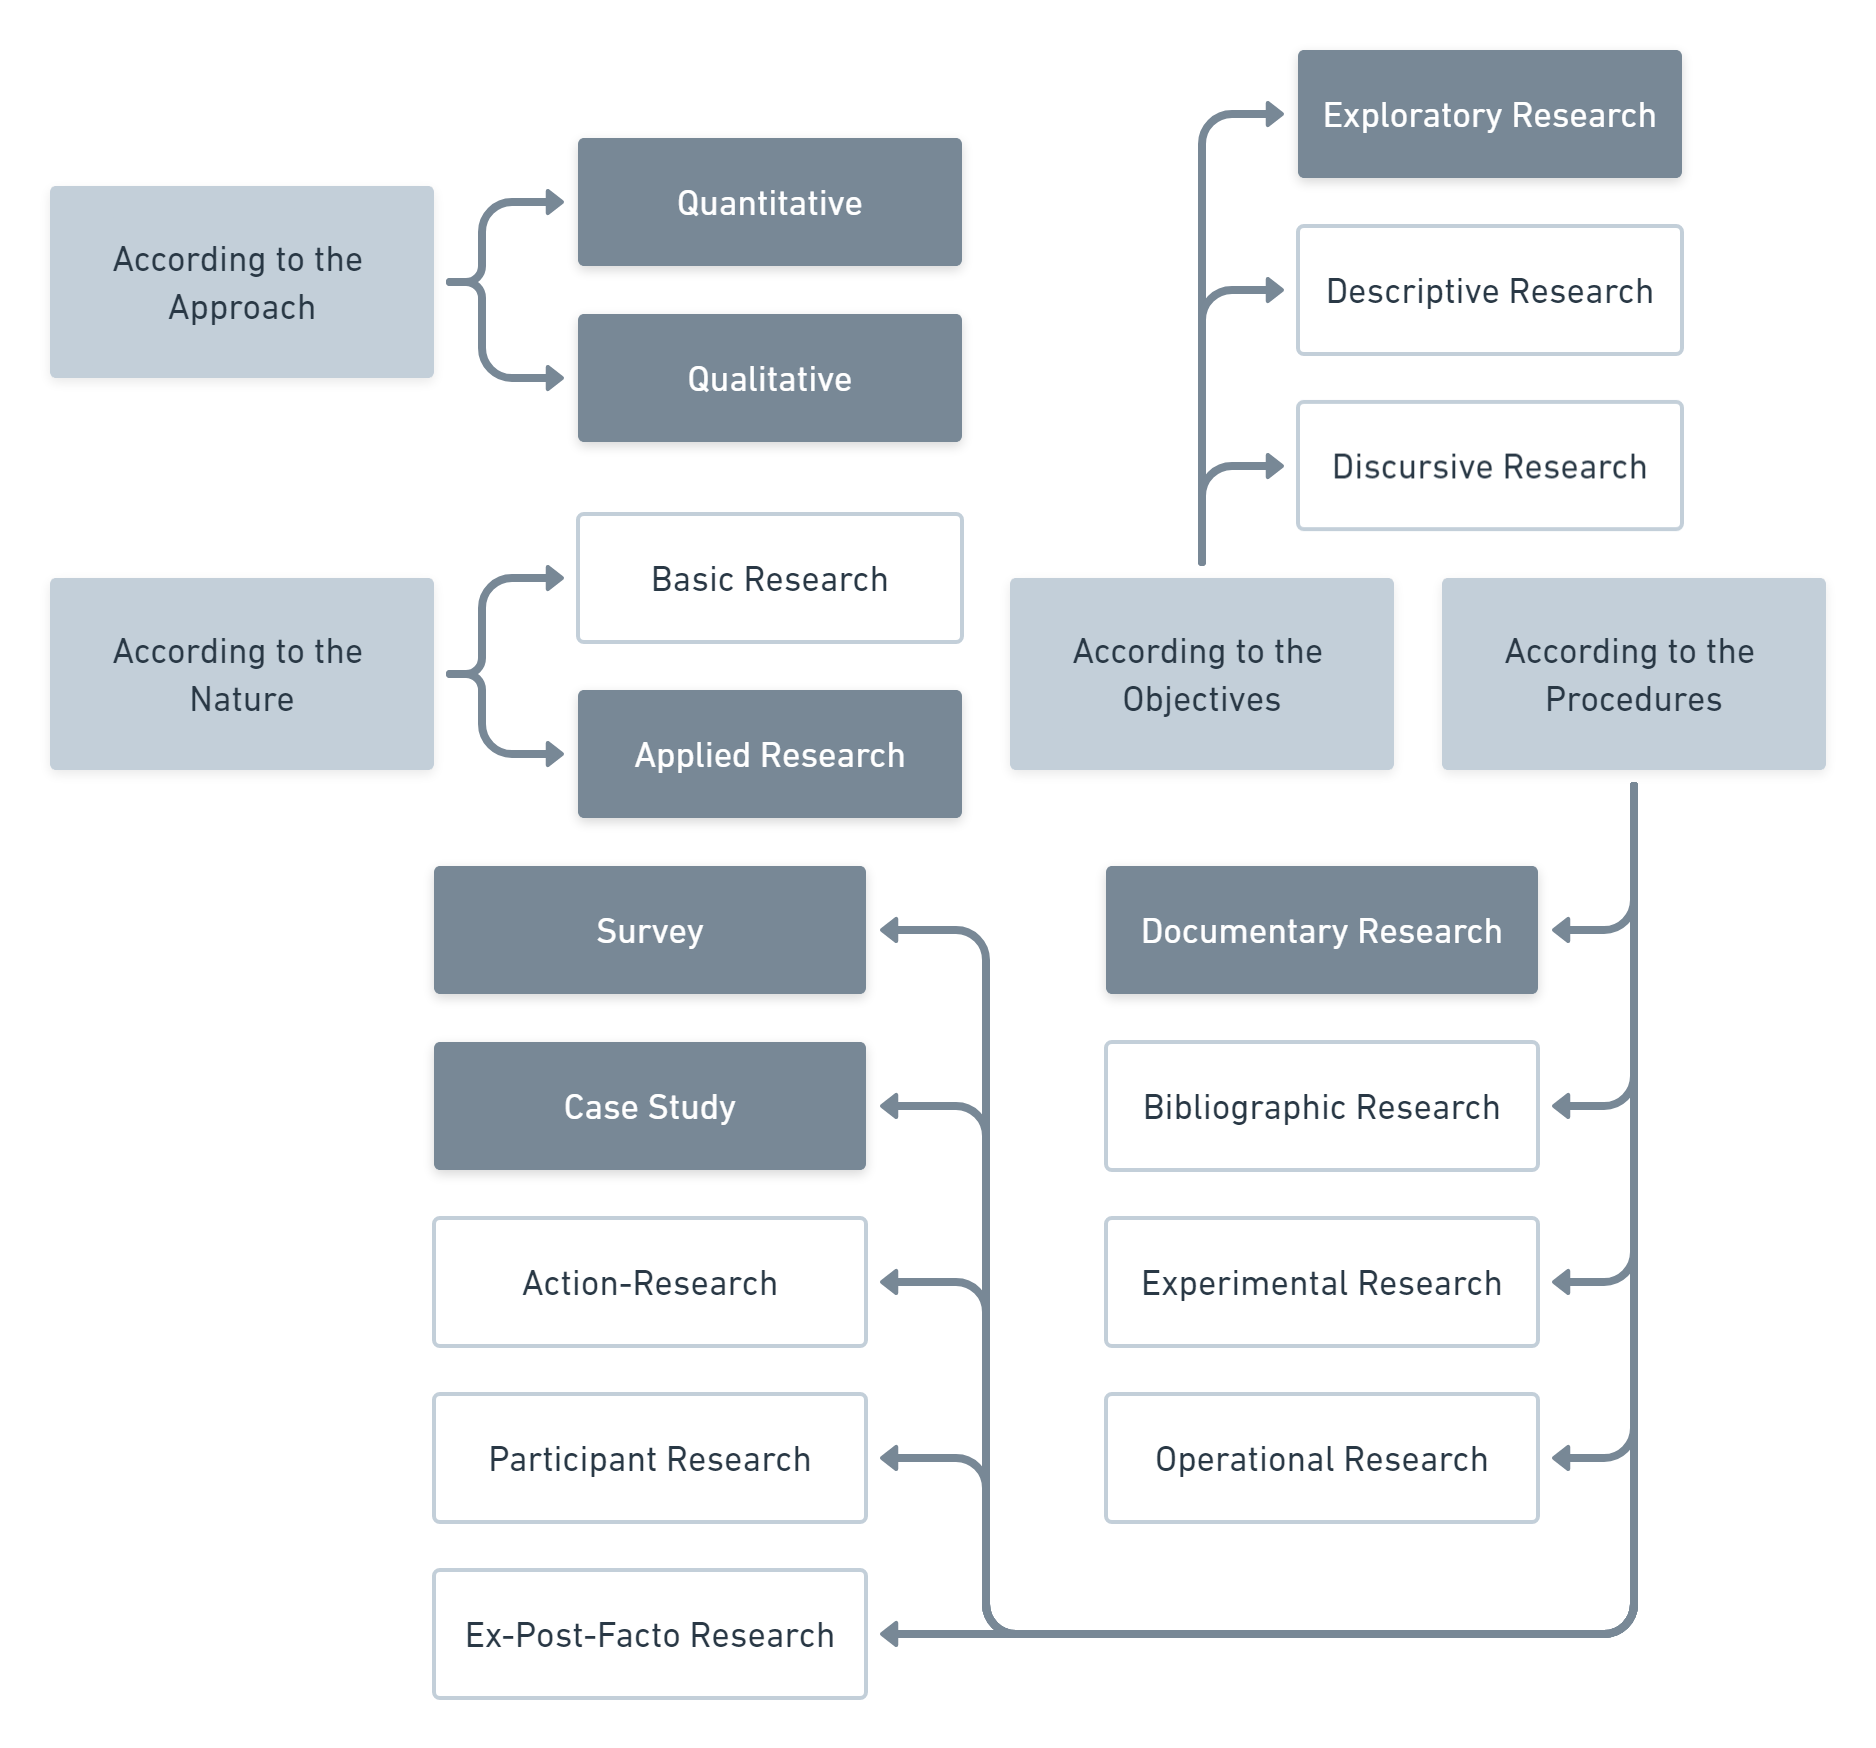
\includegraphics[width=16cm]{img/2-Research Classification@2x.png}
  \end{center}
  \fonte{Adapted from \cite{Prodanov:2013}.}
\end{figure}

Looking through the nature point of view, this is an \textbf{Applied Research}. It has the goal of generating knowledge to the solution of specific problems, through a practical application. It is related to local interests and often has a new process or product as a result.

From the objectives point of view, it is classified as an \textbf{Exploratory Research}, since one of its goals is to discover more information about what is being investigated, and maybe finding a new type of approach to the subject. This type of research generally takes the form of bibliographic research and \textbf{Case Studies}. The former doesn't apply to this study, though, because the final product won't be heavily inspired on white literature. Only the latter applies, because researches of this nature are more focused on the immediate application of knowledge in a circumstantial reality, emphasizing the development of theories.

However, the product will certainly be inspired by grey literature, meaning it fits as a \textbf{Documentary Research}. It is similar to bibliographic research, but the main difference between them is the nature of their sources. While bibliographic research makes fundamental use of contributions from various authors on a given subject, documentary research is based on materials that have not yet received an analytical treatment or that can be reworked according to the research objectives.

According to the technical procedures, this research also features a \textbf{Survey}. They are much more suitable for descriptive rather than explanatory studies. They are inappropriate for the deepening of more complex psychological and psychosocial aspects, but very effective for less delicate problems, for example, electoral preference and consumer behavior. The latter is much more aligned with this study than the former. Surveys are very useful for the study of opinions and attitudes, but little indicated in the study of problems referring to complex social structures. How this technique was applied in the scope of this work is described in detail in \Cref{survey}.

Through the approach point of view, the research is both \textbf{Quantitative}, meaning translating opinions and information into numbers to classify and analyze them. And also \textbf{Qualitative}, because some parts of the study can't be quantified, and must be understood subjectively. An example would be to receive written, detailed feedback from a target-user through the survey.

\section{Research Design}\label{sec:met-3}

In order to conduct the study correctly, a research design was created. The activities are grouped in five phases:
\begin{inparaenum}[(1)]
  \item gather information;
  \item begin development;
  \item write term paper;
  \item develop;
  \item evaluate.
\end{inparaenum}
They are all described in this section and can also be observed in \Cref{fig:research-design}.

\begin{figure}[!htb]
  \caption{Research Design}\label{fig:research-design}
  \begin{center}
    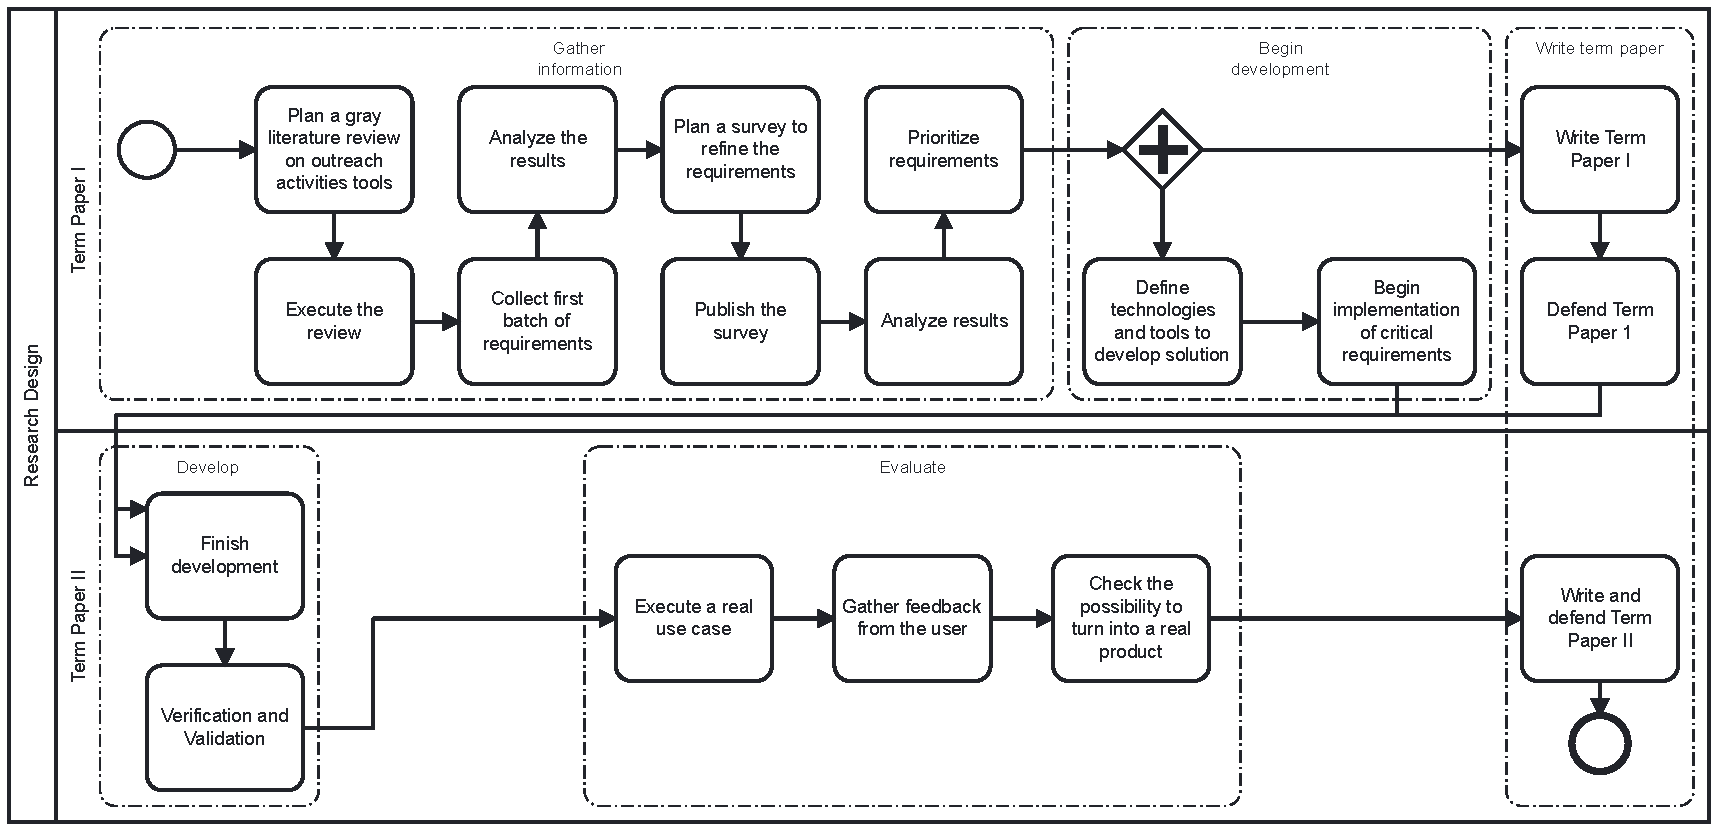
\includegraphics[width=16cm]{img/2-research design.pdf}
  \end{center}
  \fonte{Author.}
\end{figure}

The \textbf{gather information} group aims to create two tangible artifacts: the grey literature systematic review and the survey to better understand the scope of the goal product and most importantly collect a list of well defined requirements.

The \textbf{begin development} group is where the implementation and the term paper writing begins. This is where the technologies used throughout the development of the product are defined. The most important requirements should already be implemented as well.

Next, there is the \textbf{write term paper} group, in which both first and second term papers are going to be written and defended. It is important to notice that the first work will be written while the initial \ac{MVP} implementation is on going.

Continuing to the next milestone, is the \textbf{develop} group, where it is planned to finish the product development. After that, in the \textbf{evaluate} group, is where the real use case will be ran, and the feedback from it, analyzed. If all goes well, the product might turn into a real solution, adopted by the university to be used.

\section{Research Schedule}\label{sec:met-schedule}

In order to have a clear vision of the steps required to run this study, a timeline was created describing what will be done by month until the expected ending of the research. Refer to \Cref{tbl:schedule} for the full overview of what was planned.

\begin{table}[!htb]
  \centering
  \caption{Research Schedule}
  \label{tbl:schedule}
  \scriptsize
  \begin{tabular}{p{4cm}|l|lllll|lll}
    \bottomrule
    \rowcolor[rgb]{0.753,0.753,0.753} \multicolumn{1}{c|}{{\cellcolor[rgb]{0.753,0.753,0.753}}}                                       & \multicolumn{1}{c|}{\textbf{2021/2}} & \multicolumn{5}{c|}{\textbf{2022/1}} & \multicolumn{3}{c|}{\textbf{2022/2}}                                                                                                                                                                                                                                           \\
    \hhline{>{\arrayrulecolor[rgb]{0.753,0.753,0.753}}->{\arrayrulecolor{black}}---------|}
    \rowcolor[rgb]{0.753,0.753,0.753} \multicolumn{1}{c|}{\multirow{-2}{*}{{\cellcolor[rgb]{0.753,0.753,0.753}}\textbf{ Activities}}} & \textbf{Nov - Mar}                   & \multicolumn{1}{c}{\textbf{Apr}}     & \textbf{May}                         & \textbf{Jun}                         & \multicolumn{1}{l}{\textbf{Jul}}     & \textbf{Aug}                         & \textbf{Sep Oct Nov}                 & \textbf{Dec}                         & \multicolumn{1}{c|}{\textbf{Jan}}    \\
    \hline
    \rowcolor[rgb]{0.914,0.914,0.914} Plan and execute systematic review in the grey literature                                       & {\cellcolor[rgb]{0.753,0.753,0.753}} &                                      &                                      &                                      &                                      &                                      &                                      &                                      &                                      \\
    Plan and execute survey with target users                                                                                         &                                      & {\cellcolor[rgb]{0.753,0.753,0.753}} &                                      &                                      &                                      &                                      &                                      &                                      &                                      \\
    \rowcolor[rgb]{0.914,0.914,0.914} Analyze results from previous steps and map requirements                                        &                                      & {\cellcolor[rgb]{0.753,0.753,0.753}} & {\cellcolor[rgb]{0.753,0.753,0.753}} &                                      &                                      &                                      &                                      &                                      &                                      \\
    Plan and start tool development                                                                                                   &                                      &                                      & {\cellcolor[rgb]{0.753,0.753,0.753}} & {\cellcolor[rgb]{0.753,0.753,0.753}} &                                      &                                      &                                      &                                      &                                      \\
    \rowcolor[rgb]{0.914,0.914,0.914} Write Term Paper I                                                                              &                                      &                                      &                                      & {\cellcolor[rgb]{0.753,0.753,0.753}} & {\cellcolor[rgb]{0.753,0.753,0.753}} & {\cellcolor[rgb]{0.753,0.753,0.753}} &                                      &                                      &                                      \\
    Defend Term Paper I                                                                                                               &                                      &                                      &                                      &                                      &                                      & {\cellcolor[rgb]{0.753,0.753,0.753}} &                                      &                                      &                                      \\
    \rowcolor[rgb]{0.914,0.914,0.914} Continue the development of the tool                                                            &                                      &                                      &                                      &                                      &                                      & {\cellcolor[rgb]{0.753,0.753,0.753}} & {\cellcolor[rgb]{0.753,0.753,0.753}} & {\cellcolor[rgb]{0.753,0.753,0.753}} &                                      \\
    Execute a real use case on the tool                                                                                               &                                      &                                      &                                      &                                      &                                      &                                      &                                      & {\cellcolor[rgb]{0.753,0.753,0.753}} &                                      \\
    \rowcolor[rgb]{0.914,0.914,0.914} Write Term Paper II                                                                             &                                      &                                      &                                      &                                      &                                      &                                      &                                      & {\cellcolor[rgb]{0.753,0.753,0.753}} & {\cellcolor[rgb]{0.753,0.753,0.753}} \\
    Defend Term Paper II                                                                                                              &                                      &                                      &                                      &                                      &                                      &                                      &                                      &                                      & {\cellcolor[rgb]{0.753,0.753,0.753}} \\
    \toprule
  \end{tabular}
  \fonte{Author.}
\end{table}

\section{Chapter Summary}\label{sec:met-4}

This chapter provided an idea of how the methodology is defined for the study and how the research can be classified. In addition, the created research design was presented, showcasing the different planned processes for the future and those that have already been executed. \Cref{background} describes all the information and background necessary for the success of this work, while also assisting the reader in better understanding the research methodology previously described.